%!TEX root = ../out/12-Quantum-SL.tex

\usepackage{pgfplots}

\begin{document}
	
	
	\mytitle{Quantum}{Quantum algorithms}
	
	\section{Introduction}
	
	\begin{frame}
		\frametitle{A bit of information}
		
		\only<1>{ 
			Deterministic / classical bit
			
			\begin{center}
			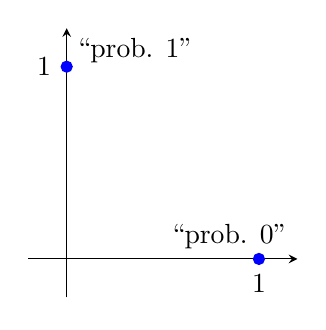
\begin{tikzpicture}
				\begin{axis}[
					width=5cm,height=5cm,
					axis lines = middle,
					xtick distance=1,
					ytick distance=1,
					xmin=-0.2,xmax=1.2,
					ymin=-0.2,ymax=1.2,
					xlabel = ``prob. 0'',
					ylabel = ``prob. 1''
					]
					\addplot[
					only marks,
					%scatter,
					mark size = 2pt,
					color=blue
					]
					coordinates {
						(0,1)(1,0)
					};
				\end{axis}
			\end{tikzpicture}
			\end{center}
		}
		\only<2>{
			Random / probabilistic bit
			
			\begin{center}
			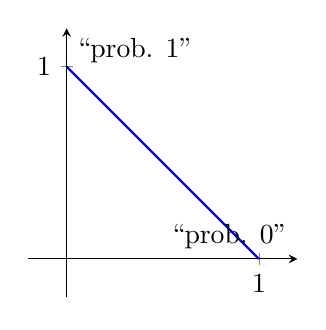
\begin{tikzpicture}
				\begin{axis}[
					width=5cm,height=5cm,
					axis lines = middle,
					xtick distance=1,
					ytick distance=1,
					xmin=-0.2,xmax=1.2,
					ymin=-0.2,ymax=1.2,
					xlabel = ``prob. 0'',
					ylabel = ``prob. 1''
					]
					\addplot[
					domain=0:1,
					samples=3,
					style=thick,
					color=blue
					]
					{1-x};
				\end{axis}
			\end{tikzpicture}
			\end{center}
		}
		\only<3>{
			Quantum bit
			
			\begin{center}
			\begin{tikzpicture}
				\begin{axis}[
					width=8cm,height=8cm,
					axis lines = middle,
					xtick distance=1,
					ytick distance=1,
					xmin=-1.2,xmax=1.2,
					ymin=-1.2,ymax=1.2,
					xlabel = ``prob. 0'',
					ylabel = ``prob. 1''
					]
					\addplot[
					domain=-1:1,
					samples=2,
					style=very thick,
					color=blue
					]
					{2};
					\draw[blue, thick]  (axis cs:0,0) circle[radius=100];
				\end{axis}
			\end{tikzpicture}
			\end{center}
		}
		
	\end{frame}
	
	\begin{frame}
		\frametitle{Quantum bit: properties}
		
		A quantum bit is in a \alert{superposition} of 0 and 1, described by two complex amplitudes $\alpha, \beta\in \mathbb{C}$:
		\begin{align*}
			\alpha |0\rangle + \beta |1\rangle
		\end{align*}
		such that $|\alpha|^2 + |\beta|^2 = 1$.
		
		\medskip
		As soon as we read a quantum bit, the superposition collapses.\\ When we read the qubit in the standard basis $\{|0\rangle,|1\rangle\}$ its value becomes $|0\rangle$ with probability $|\alpha|^2$ and $|1\rangle$ with probability $|\beta|^2$.
	\end{frame}
	
	\begin{frame}
		\frametitle{Quantum systems: properties}
		
		A set of $n$ quantum bits can be described by $2^n$ complex numbers. These quantum bits can be \alert{entangled}, making it impossible to describe the system as the product of $n$ individual qubits.
		
		\medskip
		Reading some of these $n$ qubits collapses their state and the remainder of the system becomes instantly consistent with these new states, no matter the distance between the qubits (Einstein's \alert{spooky action at a distance}).
		
		\medskip
		Computation is done via initialization, reversible unitary transformations (quantum gates), transfer (I/O operation), and measurement (read).
		
		\pause
		\medskip
		\noindent
		\textbf{Disclaimer} Further details about the quantum circuit model of computation are skipped in this lecture. Excellent expositions by world leading experts can easily be found.
		
	\end{frame}
	
	\section{Quantum complexity}
	
	
	\begin{frame}
		\frametitle{Probabilistic and quantum complexity classes}
		
		\begin{itemize}
			\item Bounded-error probabilistic polynomial time (\alert{BPP}) is the class of decision problems solvable by a probabilistic Turing machine in polynomial time with error probability $\le 1/3$.
			\item Bounded-error quantum polynomial time (\alert{BQP}) is the class of decision problems solvable by a quantum computer in polynomial time with error probability $\le 1/3$.
		\end{itemize}
		
		\begin{center}
			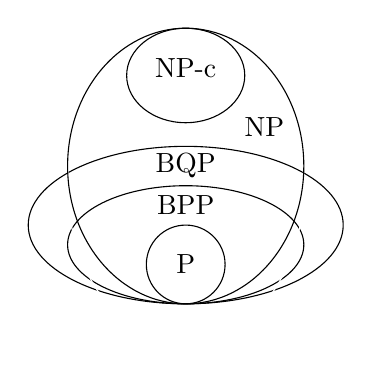
\begin{tikzpicture}
				\draw (0,0) ellipse (0.5cm and 0.5cm);
				\node at (0,0) {P};
				\draw (0,0.25) ellipse (1.5cm and 0.75cm);
				\node at (0,0.75) {BPP};
				\draw (0,0.5) ellipse (2cm and 1cm);
				\node at (0,1.25) {BQP};
				\draw[white] (0,1) ellipse (1.5cm and 2cm);
				\draw<2-> (0,1.25) ellipse (1.5cm and 1.75cm);
				\node<2-> at (1,1.75) {NP};
				\draw<2-> (0,2.4) ellipse (0.75cm and 0.6cm);
				\node<2-> at (0,2.5) {NP-c};
			\end{tikzpicture}
		\end{center}
		
		\only<2>{
			We expect that $\text{BPP} = \text{P}$.\\
			Fourier Sampling and Fourier Checking are candidates for belonging to $\text{BQP} \setminus \text{NP}$.
		}
	\end{frame}
	
	\section{Shor's algorithm}
	
	\begin{frame}
		\frametitle{Prime numbers}
		
		\begin{definition}
			A \alert{prime number} is a natural number greater than 1 that is not the product of two smaller numbers.
		\end{definition}
		\begin{block}{Examples}
			$2, 3, 5, 7, 11, 13, 17, \dots$
		\end{block}
	\end{frame}
	
	\begin{frame}
		\frametitle{Primality test}
		
		\pbDefNoPara{\textsc{PRIMES}}
		{Integer $N$}
		{Is $N$ prime?}
		
		Input size: $n = \log N$
		
		\begin{theorem}[\cite{AgrawalKS04}]
			\textsc{PRIMES} is in \P.
		\end{theorem}
		
		This is the first deterministic polynomial-time algorithm for testing whether an integer is prime.\newline
		The running time of $\tilde{O}(n^{12.5})$ has subsequently been improved to $\tilde{O}(n^{6})$. The $\tilde{O}$ notation is similar to the $O$-notation but ignores $(\log n)^{O(1)}$ factors.
	\end{frame}
	
	\begin{frame}
		\frametitle{Factoring into primes}
		
		\pbDefOpt{\textsc{Integer Factorization}}
		{Integer $N$}
		{The prime factors of $N$}
		
		\begin{theorem}[\cite{BuhlerLP93}]
			\textsc{Integer Factorization} can be solved in $2^{O(n^{1/2})}$ time (and even in $2^{O(n^{1/3})}$ time if some assumptions are true).
		\end{theorem}
		
		\pbDefNoPara{\textsc{Small Integer Factor}}
		{Integers $N$, $K$}
		{Does $N$ have a factor smaller than $K$?}
		
		Current expectations:
		\begin{itemize}
			\item \textsc{Small Integer Factor} is not \NP-hard (since it belongs to $\NP \cap \coNP$)
			\item \textsc{Small Integer Factor} is not in \P.
		\end{itemize}
		
	\end{frame}
	
	\begin{frame}
		\frametitle{Factoring on a quantum computer}
		
		\begin{theorem}[\cite{Shor94}]
			There is a bounded error quantum algorithm for \textsc{Integer Factorization} with running time $O(n^3)$.
		\end{theorem}
		Using a faster integer multiplication algorithm \cite{HarveyH21} the running time improves to $O(n^2 \log n)$.\newline
		Therefore, \textsc{Small Integer Factor} $\in$ BQP.
	\end{frame}
	
	\section{Grover's algorithm}
	
	\begin{frame}
		\frametitle{Unstructured search}
		
		\pbDefOpt{\textsc{Unstructured Search}}
		{Access to a Boolean function $f(x_1,\dots,x_n)$}
		{An assignment $\alpha : \{x_1,\dots,x_n\} \rightarrow \{0,1\}$ such that $f(x_1,\dots,x_n)=1$ (if one exists)}
		
		Typically, $f$ is encoded as a Boolean circuit.
		
		\begin{theorem}[\cite{Grover96}]
			There is a bounded error quantum algorithm for \textsc{Unstructured Search} that uses $O(2^{n/2})$ evaluations of $f$.
		\end{theorem}
	\end{frame}
	
	\begin{frame}
		\frametitle{SAT}
		
		\begin{corollary}
			There is a bounded error quantum algorithm for \SAT with running time $O^*(2^{n/2})$.
		\end{corollary}
		
		\begin{block}{Quantum Strong Exponential Time Hypothesis \cite{BuhrmanPS21}}
			There is no bounded error quantum algorithm that solves \SAT on $n$ variables in $O^*(2^{(1-\delta)n/2})$ time, for any $\delta > 0$.
		\end{block}
	\end{frame}
	
	\section{Quantum search by branching}
	
	\begin{frame}
		\frametitle{Search by branching}
		
		\begin{definition}
			A \alert{branching search algorithm} is a branching algorithm where the Combination step is a disjunction (OR).
		\end{definition}
		
		\begin{theorem}[\cite{Furer08} (see also \cite{ShimizuM22})]
			Let $A$ be a branching search algorithm that spends only polynomial time at each recursive call.\newline
			Let $\mu$ be a measure such that for each instance $I$, the search tree of $A$ executed on instance $I$ has at most $2^{\mu(I)}$ nodes.\newline
			Then, there is a bounded error quantum version of $A$ with running time $O^*(2^{\mu(I)/2})$.
		\end{theorem}
		
		F{\"{u}}rer's quantum algorithm needs to know $\mu$, but this can be avoided using tree size estimation \cite{AmbainisK17}
	\end{frame}
	
	\begin{frame}
		\frametitle{Quadratic speedups}
		
		Many branching algorithms get a quadratic speedup on quantum computers.
		
		\medskip
		For example, based on our $O^*(4^k)$ algorithm for \textsc{Max Leaf Spanning Tree}, we obtain a bounded error $O^*(2^k)$ time quantum algorithm for \textsc{Max Leaf Spanning Tree}.
	\end{frame}
	
	\section{Quantum search by randomized algorithms}
	
	\begin{frame}
		\frametitle{Guess and check}
		
		Assume we have access to a Boolean function $f(x_1,\dots,x_n)$ and a randomized 'guessing' algorithm $A$ that has success probability $\ge p$ of guessing values for $x_1,\dots,x_n$ such that $f(x_1,\dots,x_n)=1$.
		
		Classically, we get constant success probability after  $O(\lceil 1/p \rceil)$ executions of $A$.
		
		\begin{theorem}[\cite{BrassardHMT02}]
			There is a bounded error quantum algorithm that finds values for $x_1, \dots, x_n$ such that $f(x_1,\dots,x_n)=1$ using $O(\lceil 1/\sqrt{p} \rceil)$ executions of $A$.
		\end{theorem}
		
		NB. The algorithm does not need to know the success probability $p$ (it can be estimated on the fly).
	\end{frame}
	
	\begin{frame}
		\frametitle{Quadratic speedups}
		
		Many randomized algorithms get a quadratic speedup on quantum computers.
		
		\medskip
		For example, based on our $O^*(4^k)$ randomized algorithm for \FVS, we obtain a bounded error $O^*(2^k)$ time quantum algorithm for \FVS.
	\end{frame}
	
	\begin{frame}
		\frametitle{Further advances for solving NP-complete problem}
		
		Quantum walks provide a quadratic speedup for random walks.
		
		\medskip
		When the fastest classical algorithms use other algorithmic techniques, one strategy is to replace (parts of) the algorithm by algorithmic methods where we can leverage quadratic speedups on quantum computers.
		
		\medskip
		Quantum parameterized complexity \cite{BremnerJMMMS22}.
	\end{frame}
	
	
	\begin{frame}[t, allowframebreaks]
		\slides{\frametitle{References}}
		\printbibliography
	\end{frame}
\end{document}
